\documentclass[oneside]{ntuthesis}
\usepackage{cite} % 使連續的引用可以變成破折號\cite{newcombe2011dtam,engel2014lsd,engel2018direct} ex [4][5][6] => [4-6]
\usepackage{indentfirst}
\usepackage{times}
\usepackage{verbatim}
\usepackage{color}
\usepackage{url}
\usepackage{graphicx}
\usepackage{array}
\usepackage{wallpaper} 
\usepackage{etoolbox}
\usepackage{amsmath}
\usepackage{amssymb} % \mathbb
\usepackage{algorithm,algorithmic} %增加建立algorithm的套件
\usepackage{afterpage}

\usepackage[inline]{enumitem}
\usepackage{float}
\usepackage{notoccite}  % 引用編號時忽略圖目錄裡出現的引用 Ignore citations in captions in list of figures when numbering  https://tex.stackexchange.com/questions/36304/ignore-citations-in-captions-in-list-of-figures-when-numbering
\usepackage[T1]{fontenc} %處理超連結的字形錯誤
\usepackage{url}
\urlstyle{rm}

%% ▼▼▼▼▼▼▼▼▼▼▼▼▼▼▼▼▼▼▼▼  圖片相關  ▼▼▼▼▼▼▼▼▼▼▼▼▼▼▼▼▼▼▼
\parindent=2em
\graphicspath{{figures/}} %將圖片路徑整理到figures資料夾
%% ▲▲▲▲▲▲▲▲▲▲▲▲▲▲▲▲▲▲▲▲  圖片相關  ▲▲▲▲▲▲▲▲▲▲▲▲▲▲▲▲▲▲▲

\interfootnotelinepenalty=10000 % 防止footnote分頁
\usepackage{fancyhdr} % 借用此套件來擺放浮水印  設定頁首頁尾用的套件

%% ▼▼▼▼▼▼▼▼▼▼▼▼▼▼▼▼▼▼▼▼  數學相關  ▼▼▼▼▼▼▼▼▼▼▼▼▼▼▼▼▼▼▼
\usepackage{mathtools}
\DeclarePairedDelimiter\floor{\lfloor}{\rfloor}
\usepackage{siunitx}% degree symbol
%% ▲▲▲▲▲▲▲▲▲▲▲▲▲▲▲▲▲▲▲▲  數學相關  ▲▲▲▲▲▲▲▲▲▲▲▲▲▲▲▲▲▲▲

%% ▼▼▼▼▼▼▼▼▼▼▼▼▼▼▼▼▼▼▼▼  表格相關  ▼▼▼▼▼▼▼▼▼▼▼▼▼▼▼▼▼▼▼
\usepackage{booktabs}
\usepackage{multirow} % 表格跨欄
\usepackage{caption} 
\captionsetup[table]{skip=5pt}
\usepackage{threeparttable}
\usepackage{tabularx}
\usepackage{longtable}
\usepackage{diagbox}
\usepackage{makecell}
\usepackage{chngcntr}

\counterwithout*{table}{chapter} %book環境table編號會跑掉,用這個套件還原
\counterwithout*{figure}{chapter}
\counterwithout*{equation}{chapter}
\newcolumntype{P}[1]{>{\centering\arraybackslash}p{#1}} % 大寫P可以讓table用p時還可以置中
\renewcommand\tabularxcolumn[1]{m{#1}}
\renewcommand{\arraystretch}{2}
% \renewcommand{\arraystretch}{2.5}
%% ▲▲▲▲▲▲▲▲▲▲▲▲▲▲▲▲▲▲▲▲  表格相關  ▲▲▲▲▲▲▲▲▲▲▲▲▲▲▲▲▲▲▲

%% ▼▼▼▼▼▼▼▼▼▼▼▼▼▼▼▼▼▼▼▼  目錄行距  ▼▼▼▼▼▼▼▼▼▼▼▼▼▼▼▼▼▼▼
\usepackage{tocloft}
\setlength{\cftaftertoctitleskip}{6pt} %目錄標題行距
\setlength{\cftafterloftitleskip}{6pt}
\setlength{\cftafterlottitleskip}{6pt}
\setlength\cftbeforechapskip{0pt}
\setlength{\cftbeforesecskip}{0pt}
\setlength{\cftbeforesubsecskip}{0pt}
\renewcommand{\cftchapafterpnum}{\vspace{3pt}}
\renewcommand{\cftfigafterpnum}{\vskip0pt}
\renewcommand{\cfttabafterpnum}{\vskip0pt}
\setlength{\cfttabnumwidth}{3em}
\setlength{\cftfignumwidth}{3em}
%% ▲▲▲▲▲▲▲▲▲▲▲▲▲▲▲▲▲▲▲▲  目錄行距  ▲▲▲▲▲▲▲▲▲▲▲▲▲▲▲▲▲▲▲  

%% ▼▼▼▼▼▼▼▼▼▼▼▼▼▼▼▼▼▼▼▼  中文章節  ▼▼▼▼▼▼▼▼▼▼▼▼▼▼▼▼▼▼▼
\usepackage{titlesec}
\usepackage{titletoc}
\usepackage{xCJKnumb}
\newcommand{\tocformat}{%
	\titleformat{\chapter}
		{\centering\fontsize{16pt}{16}\bfseries}
		{第\,\xCJKnumber{\thechapter}\,章}{1em}{}
	
	\titleformat{\section}{\fontsize{14pt}{14.4pt}\selectfont\bfseries}{\thesection}{1em}{}
	\titleformat{\subsection}{\fontsize{12pt}{13.2pt}\selectfont\bfseries}{\thesubsection}{1em}{}
	\titlespacing{\chapter}{0pt}{6pt}{6pt}
	\titlespacing{\section}{0pt}{3pt}{3pt}
	\titlespacing{\subsection}{0pt}{0pt}{0pt}
}
\newcommand{\tocformatbib}{%
	\titleformat{\chapter}
		{\centering\fontsize{16pt}{16}\bfseries}
		{第\,\xCJKnumber{\thechapter}\,章}{1em}{}	
}
\newcommand{\toccontentsformat}{ %目錄格式
	\titlecontents{chapter}[0pt]{\addvspace{1.5pt}\filright}
				{\contentspush{第\xCJKnumber{\thecontentslabel}章\quad}}
				{}{\titlerule*[8pt]{.}\contentspage}
}
\newcommand{\tocformatappendix}{
	\setcounter{section}{0}
	\setcounter{subsection}{0}
}
%% ▲▲▲▲▲▲▲▲▲▲▲▲▲▲▲▲▲▲▲▲  中文章節  ▲▲▲▲▲▲▲▲▲▲▲▲▲▲▲▲▲▲▲  

%% ▼▼▼▼▼▼▼▼▼▼▼▼▼▼▼▼▼▼▼▼  目錄相關  ▼▼▼▼▼▼▼▼▼▼▼▼▼▼▼▼▼▼▼ 
\renewcommand{\contentsname}{\hfill\fontsize{16pt}{16} 目錄\hfill}
\renewcommand{\listfigurename}{\hfill\fontsize{16pt}{16}\bfseries 圖目錄\hfill}
\renewcommand{\listtablename}{\hfill\fontsize{16pt}{16}\bfseries 表目錄\hfill}
\renewcommand{\figurename}{}
\renewcommand{\thefigure}{圖\arabic{figure}}
\renewcommand{\tablename}{}
\renewcommand{\thetable}{表\arabic{table}}
\renewcommand{\bibname}{參考文獻}
\renewcommand{\theequation}{\arabic{equation}}
%% ▲▲▲▲▲▲▲▲▲▲▲▲▲▲▲▲▲▲▲▲  目錄相關  ▲▲▲▲▲▲▲▲▲▲▲▲▲▲▲▲▲▲▲  

%% ▼▼▼▼▼▼▼▼▼▼▼▼▼▼▼▼▼▼▼▼  浮水印    ▼▼▼▼▼▼▼▼▼▼▼▼▼▼▼▼▼▼▼
\pagestyle{fancy} % 啟動 fancy header/footer 套件
\setlength{\headheight}{15pt}
\fancyheadoffset{15pt}
\renewcommand{\headrulewidth}{0pt} % header 的直線; 0pt 則無線
%
% this file is encoded in utf-8
% v2.0 (Apr. 5, 2009)
% 如果浮水印不是全篇需要,請把下列介於 >>> 與 <<<
% 的「全篇浮水印專用碼」關掉 (行首加百分號)
% 參考自 Keith Reckdahl 寫的 "Using Imported Graphics in LATEX2e" (epslatex.pdf) p.39
% 如果只有特定頁需要浮水印
% 則依該頁屬性使用下列之一的命令 
% 普通頁命令 \thispagestyle{WaterMarkPage}
% plain 頁命令 \thispagestyle{PlainWaterMarkPage}
% empty 頁命令 \thispagestyle{EmptyWaterMarkPage}


% 將重複使用的浮水印章
% 圖檔是 my_watermark.xxx
% 副檔名可以不加,可以是 latex 系統能處裡的任何格式:pdf, gif, png, jpg, eps, ...
% 某些圖檔格式在某些工作流程可能需要作前置處裡。
% 例如,pdflatex 無法直接處理 eps 檔
%  latex + dvipdfmx 無法直接處理 pdf, gif, png, jpg, 需要用 ebb 小工具程式
%  對圖檔產生 .bb 對應檔。
%
% 寬為 5.1 cm
\newsavebox{\mywatermark}
\sbox{\mywatermark}{
\includegraphics[keepaspectratio,width=8cm]{watermark/CCU.pdf}}


% 將 central header 擺放浮水印的巨集指令
\newcommand{\PlaceWaterMark}{\fancyhead[C]{\setlength{\unitlength}{1in}%
\begin{picture}(0,0)%
\put(-1.6,-6.25){\usebox{\mywatermark}} % 圖檔擺放的位置座標
\end{picture}}
}

\fancyhead{}  % reset left, central, right header to empty
% 如果不需整篇論文都要浮水印
% 則下面  >>> 與 <<< 之間的程式碼請關閉
% >>> 全篇浮水印
\PlaceWaterMark  % 每一頁都有浮水印 (除了 plain、empty 頁以外)

% 重新定義 plain 頁面
% 每張 plain 頁面 (每一章的第一頁) 也加浮水印

\fancypagestyle{plain}{
\fancyhead{}
\PlaceWaterMark
\fancyfoot{}
\fancyfoot[C]{\thepage}
\renewcommand{\headrulewidth}{0pt}
\renewcommand{\footrulewidth}{0pt}
}
% <<< 全篇浮水印

% 如果只有一、兩頁需要有浮水印
% 可以在該頁 (有頁碼) 使用 \thispagestyle{WaterMarkPage}
% 此命令不影響原有的 header、footer
\fancypagestyle{WaterMarkPage}{
\PlaceWaterMark
}

% 如果只有一、兩頁 plain 頁需要有浮水印 (如 摘要、自傳等)
% 可以在該頁 (有頁碼) 使用 \thispagestyle{PlainWaterMarkPage}
% 只有頁碼與浮水印,沒有其他的 header、footer
% 等同於 plain page style + water mark
\fancypagestyle{PlainWaterMarkPage}{
\fancyhead{}
\PlaceWaterMark
\fancyfoot{}
\fancyfoot[C]{\thepage}
\renewcommand{\headrulewidth}{0pt}
\renewcommand{\footrulewidth}{0pt}
}

% 如果只有一、兩頁 empty 頁需要有浮水印 (如封面、書名頁)
% 可以在該頁 (無頁碼) 使用 \thispagestyle{EmptyWaterMarkPage}
% 等同於 empty page style + water mark
\fancypagestyle{EmptyWaterMarkPage}{
\fancyhead{}
\PlaceWaterMark
\fancyfoot{}
\renewcommand{\headrulewidth}{0pt}
\renewcommand{\footrulewidth}{0pt}
}

%% ▲▲▲▲▲▲▲▲▲▲▲▲▲▲▲▲▲▲▲▲  浮水印    ▲▲▲▲▲▲▲▲▲▲▲▲▲▲▲▲▲▲▲  

%% ▼▼▼▼▼▼▼▼▼▼▼▼▼▼▼▼▼▼▼▼  編號相關  ▼▼▼▼▼▼▼▼▼▼▼▼▼▼▼▼▼▼▼
\newenvironment{descitemize} % a mixture of description and itemize
  {\begin{description}[
	topsep=0pt, 
	parsep=0pt, 
	itemsep=0pt, 
	labelsep=3pt, 
	leftmargin=0pt, 
	listparindent=1pt, 
	before=\let\makelabel\descitemlabel]}
  {\end{description}}
\newcommand{\descitemlabel}[1]{%
  \textbullet\ \textbf{#1}%
}
\setlist[enumerate]{
	topsep=0pt, 
	parsep=0pt, 
	itemsep=0pt, 
	labelsep=3pt, 
	leftmargin=*, 
	% itemindent=!, 
	listparindent=2em,
	label=\textbf{\arabic*.}
}
\setlist[itemize]{
	topsep=0pt, 
	parsep=0pt, 
	itemsep=0pt, 
	labelsep=3pt, 
	leftmargin=*, 
	% itemindent=1em, 
	listparindent=2em,
}
%% ▲▲▲▲▲▲▲▲▲▲▲▲▲▲▲▲▲▲▲▲  編號相關  ▲▲▲▲▲▲▲▲▲▲▲▲▲▲▲▲▲▲▲

%% ▼▼▼▼▼▼▼▼▼▼▼▼▼▼▼▼▼▼▼▼  演算法相關  ▼▼▼▼▼▼▼▼▼▼▼▼▼▼▼▼▼▼▼
\renewcommand{\algorithmiccomment}[1]{\hspace{1em}~//\emph{#1}} %修改演算法的註解格式
%% ▲▲▲▲▲▲▲▲▲▲▲▲▲▲▲▲▲▲▲▲  演算法相關  ▲▲▲▲▲▲▲▲▲▲▲▲▲▲▲▲▲▲▲

% Using the tex-text mapping for ligatures etc.
\defaultfontfeatures{Mapping=tex-text}

% Set the default fonts
\setmainfont{Times New Roman}
\setCJKmainfont[AutoFakeBold=true, AutoFakeSlant=.2]{標楷體} %for Windows OS
% \setCJKmainfont[AutoFakeBold=true, AutoFakeSlant=.2]{楷體-繁} % for MacOS
% \setCJKmainfont[AutoFakeBold=true, AutoFakeSlant=.2]{DFKai-SB} %for Ubuntu
% Windows 字型
% > dir %windir%\fonts

\ifdefined\withwatermark
  \CenterWallPaper{0.174}{watermark.pdf}
  \setlength{\wpXoffset}{6.1725cm}
  \setlength{\wpYoffset}{10.5225cm}
\fi

% digital object identifier
\ifdefined\withdoi
  \insertdoi
\fi

\makeatletter
\AtBeginDocument{
  \hypersetup{
    pdftitle={\@titleen},
    pdfauthor={\@authoren},
    pdfsubject={\@typeen{} \@classen},
    pdfkeywords={\@keywordsen}
  }
}

% 這些要放在hyperref套件前面,要不然lot的行距會壞掉
\patchcmd{\@chapter}
  {\addtocontents{lof}{\protect\addvspace{10\p@}}}
  {}
  {}{}
\patchcmd{\@chapter}
  {\addtocontents{lot}{\protect\addvspace{10\p@}}}
  {}
  {}{}

\makeatother

\usepackage[hidelinks,linktoc=all]{hyperref} %可建立註解以及參考文獻網址的超連結
\hypersetup{%
	colorlinks=false,% switch on coloured instead of framed links
	linkcolor=black,% main link color (e.g. for the ToC)182,48,23
}   

\newcommand{\blankpage}{ %插入空白頁面
    \null
    \thispagestyle{empty}%
    \addtocounter{page}{-1}%
    \newpage}


\newcommand{\setchapleaders}[1]{
	\addtocontents{toc}{%
		\protect\renewcommand{\protect\cftchapdotsep}{#1}% set chapter leaders
	}
}

% Your information goes here
% author: Tz-Huan Huang [http://www.csie.ntu.edu.tw/~tzhuan]

% ----------------------------------------------------------------------------
% "THE CHOCOLATE-WARE LICENSE":
% Tz-Huan Huang wrote this file. As long as you retain this notice you
% can do whatever you want with this stuff. If we meet some day, and you think
% this stuff is worth it, you can buy me a chocolate in return Tz-Huan Huang
% ----------------------------------------------------------------------------

% Syntax: \var{English}{Chinese}
\university{National Chung Cheng University}{國立中正大學}
\address{Chiayi, Taiwan, Republic of China}{}
\college{College of Engineering}{工學院}
\institute{Electrical Engineering}{電機工程研究所}
\title{Recommendation System}{推薦系統}
\author{Jih-Hsiang Wu}{吳日翔}
\studentid{610415130}
\advisor{Alan Lu, Ph. D.}{劉立頌 \hspace*{6pt} 博士}
\coadvisor{}{}%共同指導
\defenseyear{2023}{111}
\defensemonth{July}{7}
\defenseday{28}
\doi{doi:10.6342/NTU2017XXXXX}
\keywords{到thesisvar.tex裡修改keyword, keyword, keyword, keyword}{到thesisvar.tex裡修改keyword, keyword, keyword, keyword} 


\begin{document}
	
	\frontmatter
	\makecover
	\afterpage{\blankpage}
	\toccontentsformat
	\addtocontents{toc}{\protect \hbox to \textwidth{{章節}~\hfill{頁碼}}} %要放在 \begin{acknowledgementszh}
感謝\ldots
\end{acknowledgementszh}

% \begin{acknowledgementsen}
% I'm glad to thank\ldots 
% \end{acknowledgementsen}
 \begin{abstractzh}
許多線上學習資源現今公開在網路上,像是開方式課程(Open Coures Ware, OCW)或是大規模開放線上課堂(Massive Open Online Course, MOOC),學習者可能會碰到過度選擇(Overchoice)問題。本研究提供不採用使用者資料之標籤式推薦演算法來解決過度選擇問題。在本系統中,採用了Yake模型進行關鍵字生成以及DBPedia之本體論架構增加標籤之多樣性,針對國立中正大學之課程進行推薦,並利用標籤相似度分析推薦給使用者其他校外學習資源。在實驗中,本研究採用了AB測試來進行驗證並證明使用者對於本研究架構較其他架構有高度的接受性。

\bigbreak
\noindent \textbf{關鍵字:}{\, \makeatletter \@keywordszh \makeatother}
\end{abstractzh}

\begin{abstracten}
Many extracurricular resources have been published on the internet, like MOOCs and OCW, so the learner who is interested in specific knowledge will encounter the over-choice problem. This work presents a tag-based recommendation system without user profiles to approach over-choice problems. In our system, we use the YAKE model to generate keywords and the Dbpedia ontology database to increase the diversity of the keywords for courses offered by National Chung Cheng University. The system will recommend other courses and extracurricular MOOCs with similar tags to the learner. In the experiment, we use the AB testing method to show that our system can recommend the courses to learners with higher satisfaction than other methods.

\bigbreak
\noindent \textbf{Keywords:}{\, \makeatletter \@keywordsen \makeatother}
\end{abstracten}

\begin{comment}
\category{I2.10}{Computing Methodologies}{Artificial Intelligence --
Vision and Scene Understanding} \category{H5.3}{Information
Systems}{Information Interfaces and Presentation (HCI) -- Web-based
Interaction.}

\terms{Design, Human factors, Performance.}

\keywords{Region of interest, Visual attention model, Web-based
games, Benchmarks.}
\end{comment}
 前面
	\begin{acknowledgementszh}
感謝\ldots
\end{acknowledgementszh}

% \begin{acknowledgementsen}
% I'm glad to thank\ldots 
% \end{acknowledgementsen}

	\begin{abstractzh}
許多線上學習資源現今公開在網路上,像是開方式課程(Open Coures Ware, OCW)或是大規模開放線上課堂(Massive Open Online Course, MOOC),學習者可能會碰到過度選擇(Overchoice)問題。本研究提供不採用使用者資料之標籤式推薦演算法來解決過度選擇問題。在本系統中,採用了Yake模型進行關鍵字生成以及DBPedia之本體論架構增加標籤之多樣性,針對國立中正大學之課程進行推薦,並利用標籤相似度分析推薦給使用者其他校外學習資源。在實驗中,本研究採用了AB測試來進行驗證並證明使用者對於本研究架構較其他架構有高度的接受性。

\bigbreak
\noindent \textbf{關鍵字:}{\, \makeatletter \@keywordszh \makeatother}
\end{abstractzh}

\begin{abstracten}
Many extracurricular resources have been published on the internet, like MOOCs and OCW, so the learner who is interested in specific knowledge will encounter the over-choice problem. This work presents a tag-based recommendation system without user profiles to approach over-choice problems. In our system, we use the YAKE model to generate keywords and the Dbpedia ontology database to increase the diversity of the keywords for courses offered by National Chung Cheng University. The system will recommend other courses and extracurricular MOOCs with similar tags to the learner. In the experiment, we use the AB testing method to show that our system can recommend the courses to learners with higher satisfaction than other methods.

\bigbreak
\noindent \textbf{Keywords:}{\, \makeatletter \@keywordsen \makeatother}
\end{abstracten}

\begin{comment}
\category{I2.10}{Computing Methodologies}{Artificial Intelligence --
Vision and Scene Understanding} \category{H5.3}{Information
Systems}{Information Interfaces and Presentation (HCI) -- Web-based
Interaction.}

\terms{Design, Human factors, Performance.}

\keywords{Region of interest, Visual attention model, Web-based
games, Benchmarks.}
\end{comment}

	\clearpage % 換頁
	
	{
		\hypersetup{%
			pdfborder = {0 0 0}%移除超連結外的紅框框
		} 
		
		\addcontentsline{toc}{chapter}{目錄}
		\tableofcontents  
		\cleardoublepage
		\addcontentsline{toc}{chapter}{圖目錄}
		\listoffigures
		\addtocontents{lof}{\protect\hbox to \textwidth{\hspace{15pt} {圖}~\hfill{頁碼}}} %dirty hack
		\cleardoublepage
		\addcontentsline{toc}{chapter}{表目錄}
		\listoftables 
		\addtocontents{lot}{\protect\hbox to \textwidth{\hspace{15pt} {表}~\hfill{頁碼}}}
		\cleardoublepage
	}
	
	\mainmatter
	
	\tocformat
	% Your thesis goes here
	\chapter{緒論}
\label{chapter:introduction}

In recent years, many extracurricular resources have been published on the internet, like Massive Open Online Courses (MOOCs) and Open Course Ware (OCW), so learners can easily learn about any topic of interest. These learning resources that can be used at a computer without restrictions on the time and place and reduce the physical limitations while learning, and can be regarded as e-learning technology \cite{tan2008}. Many universities have provided e-learning resources. However, learners cannot quickly choose the resources to appropriate their requirements, since there are too many choices, which might decrease the learning effect. 
A tag-based recommendation system is one of the approaches to this problem. The recommendation system is an information-filtering technique that solves the over-choice problems \cite{zhang2019}. This system will analyze the properties of extracurricular resources, generate related tags, and recommend them to the learner by finding other resources with similar tags. There are some mainstream methods to implement recommendation systems: content-based filtering, collaborative filtering, and hybrid method \cite{nagarnaik2015}. The most common e-learning recommendation system is a collaborative-based filtering recommendation system, which focuses on customized recommendations based on user information \cite{ali2022}. To the best of our knowledge, there are no studies using tag-based, content-based recommendation systems without user profiles. 
In this study, we propose a tag-based recommendation system without user profiles that will recommend other courses and MOOCs provided by MIT, Coursera, and Udemy, related to courses offered by National Chung Cheng University.


	\chapter{背景知識及文獻探討}
\label{chapter:relatedWork}
\par 這裡是related work...

\begin{figure}[h!]
    \centering
    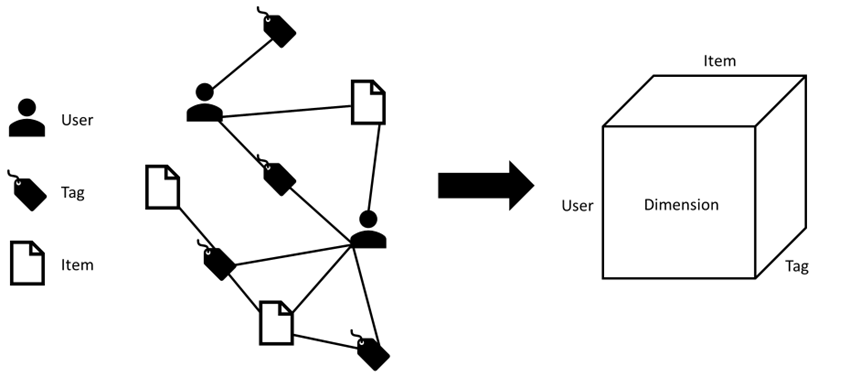
\includegraphics{threeDim.png}
    \caption{將無向三方圖表示為三維矩陣}
    \label{fig:threeDim}
\end{figure}
	\chapter{架構方法}
\label{chapter:processing}

\begin{algorithm}
    \caption{Bubble Sort}
    \begin{algorithmic}
        \renewcommand{\algorithmicrequire}{\textbf{Input:}}
        \renewcommand{\algorithmicensure}{\textbf{Output:}}
        \REQUIRE Input Array A[]
        \ENSURE  Sorted Array A[]
        \\ \textit{Initialisation} :
        \STATE int $i,j,k;$
        \STATE int $N \gets length(A);$
        \\ \textit{LOOP Process}
        \FOR {$i = 0$ to $N-1$}
            \FOR {$j = 0$ to $N-i-1$}
                \IF {($A[j] > A[j+1]$)}
                    \STATE swap($A[j]$, $A[j+1]$)
                \ENDIF
            \ENDFOR
        \ENDFOR
        \RETURN $A$ 
    \end{algorithmic} 
    \label{alg:alg1}
\end{algorithm}

\section{系統架構說明}
\label{sec:processing}

這個架構\ldots
   
	\chapter{實驗}
\label{chapter:testing}

\section{實驗方法}
\label{sec:testing_method}

\begin{table}[ht!]
    
    \caption{實驗之混淆矩陣}
    \centering

    \resizebox{\columnwidth}{!}{\begin{tabular}{|c|c|c|c|}
        \hline
        \diagbox{True}{Predicted} & \begin{tabular}[c]{@{}c@{}}Open\\ Drawer 1\end{tabular} & \begin{tabular}[c]{@{}c@{}}Open\\ Drawer 2\end{tabular} & \begin{tabular}[c]{@{}c@{}}Open\\ Drawer 3\end{tabular} \\ \hline
        Open Drawer 1 & 62\% & 0\% & 0\% \\ \hline
        Open Drawer 2 & 28\% & 35\% & 0\% \\ \hline
        Open Drawer 3 & 1\% & 15\% & 63\% \\ \hline
    \end{tabular}}
    \label{table:Exp4ConfuseMatrix}
\end{table}

\section{實驗一}
\label{sec:testing_exp1}

\begin{descitemize}
    \item[實驗目的]
    
    我們將依照\ref{sec:testing_method}節所述的方法,進行實驗。
    
    \item[實驗步驟] 
    
    實驗方法如下:

\end{descitemize}
	\chapter{結論}
\label{chapter:conclusion}
	
	\tocformatbib
	\appendix

	\backmatter

	%% 參考文獻
	\addcontentsline{toc}{chapter}{\bibname} %摘要、文獻等頁碼編進目錄
	\bibliographystyle{IEEEtran}
	\bibliography{thesis}
	%附錄 要放在\backmatter後
	\counterwithin*{section}{chapter}
	
\chapter{附錄A}
\label{chapter:appendixA}
The contents...

\chapter{附錄B}
\label{chapter:appendixB}
這裡是附錄B

\end{document}
